\documentclass[11pt,xcolor=pdflatex]{beamer}
\usepackage{newcent}
\usepackage[utf8]{inputenc}
\usepackage[czech]{babel}
\usepackage{hyperref}
\usepackage{fancyvrb}
\usepackage{appendixnumberbeamer}
\usetheme{FIT}

\newcommand\myheading[1]{%
  \par\bigskip
  {\Large#1}\par\smallskip}
  
%%%%%%%%%%%%%%%%%%%%%%%%%%%%%%%%%%%%%%%%%%%%%%%%%%%%%%%%%%%%%%%%%%

\title[Monitorování chodců pomocí dronu]{Monitorování chodců pomocí dronu}

\author[]{Vladimír Dušek}

\institute[]{Vysoké učení technické v Brně, Fakulta informačních technologií \\
Božetěchova 1/2. 612 66 Brno - Královo Pole \\
xdusek27@stud.fit.vutbr.cz}

\date{10. června 2019}

%%%%%%%%%%%%%%%%%%%%%%%%%%%%%%%%%%%%%%%%%%%%%%%%%%%%%%%%%%%%%%%%%%

\begin{document}

\frame[plain]{\titlepage}

%%%%%%%%%%%%%%%%%%%%%%%%%%%%%%%%%%%%%%%%%%%%%%%%%%%%%%%%%%%%%%%%%%

\begin{frame}\frametitle{Představení zadání}

\myheading{Cíl práce}

\begin{itemize}
    \item Vytvořit aplikaci pro monitorování chodců ve videozáznamu  pořízeným dronem.
    \begin{itemize}
		\item Je předpokládán pohled z výšky.
	\end{itemize}
\end{itemize}
	
\myheading{Dekompozice}

\begin{enumerate}
    \item Detekovat lidi v každém snímku videa.
	\item Jednotlivé osoby od sebe vzájemně rozlišit.
	\item Sledovat jejich pohyb v průběhu celého videa.
	\item Vykreslit trajektorie jejich pohybů.
\end{enumerate}

\end{frame}

%%%%%%%%%%%%%%%%%%%%%%%%%%%%%%%%%%%%%%%%%%%%%%%%%%%%%%%%%%%%%%%%%%

\begin{frame}\frametitle{Návrh aplikace}

\begin{figure}[H]
    \centering
    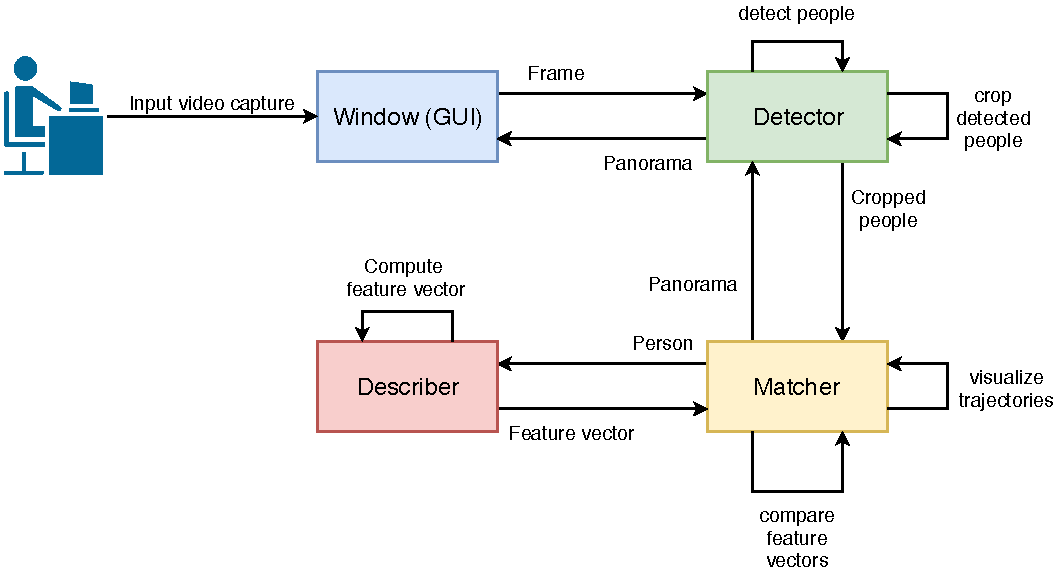
\includegraphics[width=.99\linewidth]{images/app-schema.pdf}
\end{figure}	
	
\end{frame}

%%%%%%%%%%%%%%%%%%%%%%%%%%%%%%%%%%%%%%%%%%%%%%%%%%%%%%%%%%%%%%%%%%

\begin{frame}\frametitle{Trénování detektoru}

    \begin{itemize}
        \item Detekční síť Retinanet
        \begin{itemize}
		    \item Předtrénovaný model nedokáže rozpoznat lidi z výšky.
	    \end{itemize}
        \item Stanford Drone Dataset
    \end{itemize}
    
    \begin{figure}[H]
        \centering
        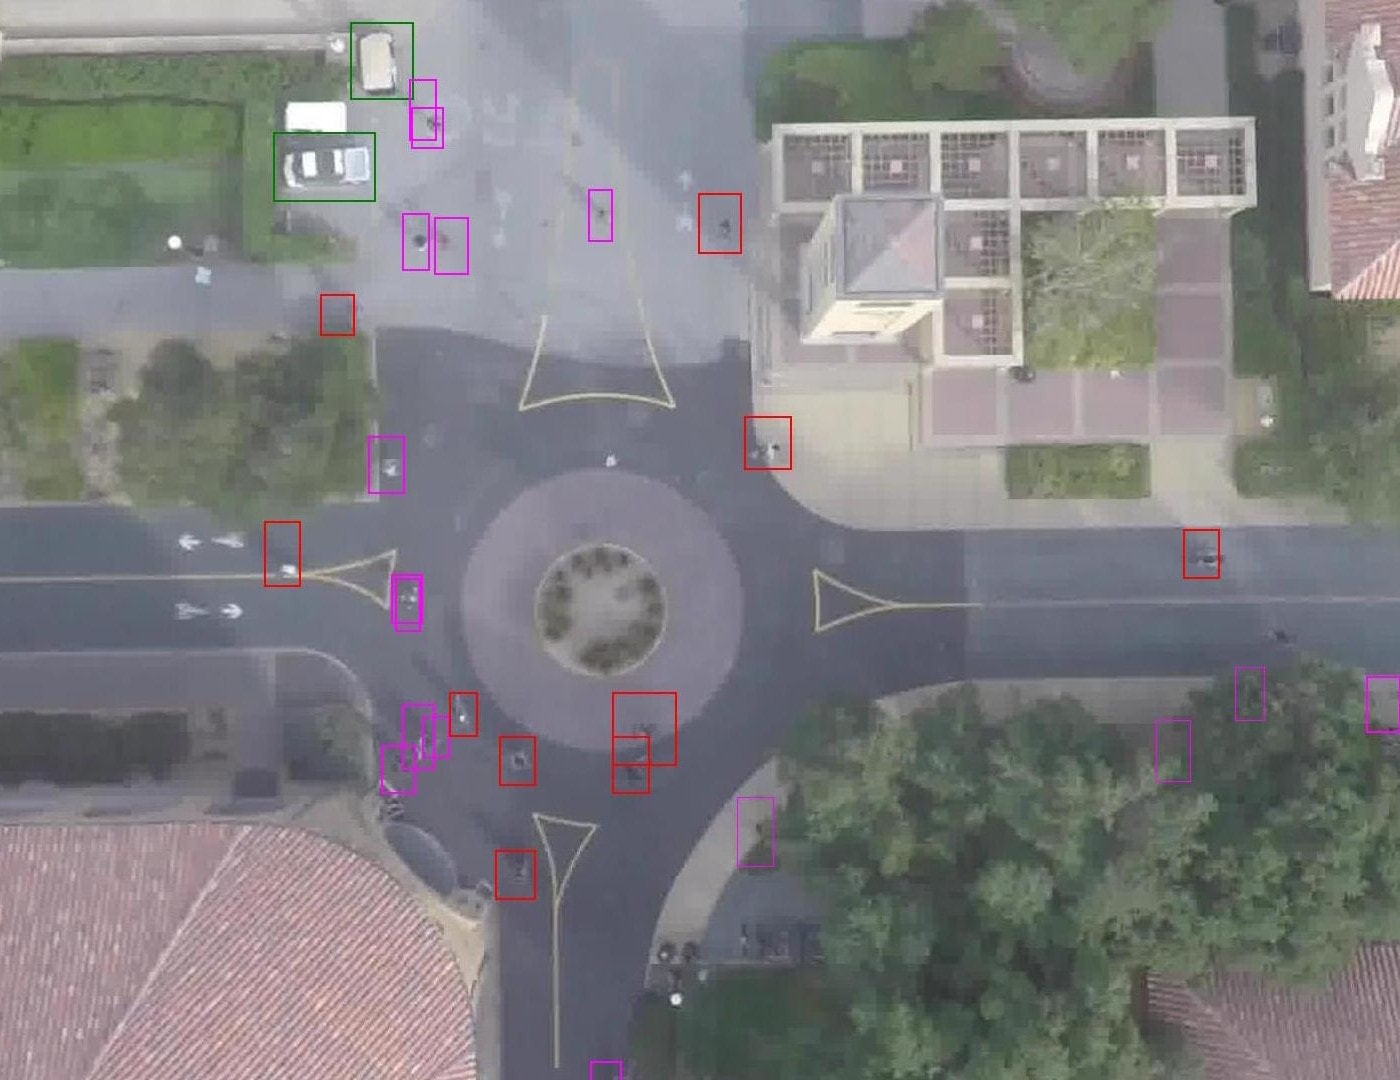
\includegraphics[width=.49\linewidth]{images/dataset_2.jpg}
        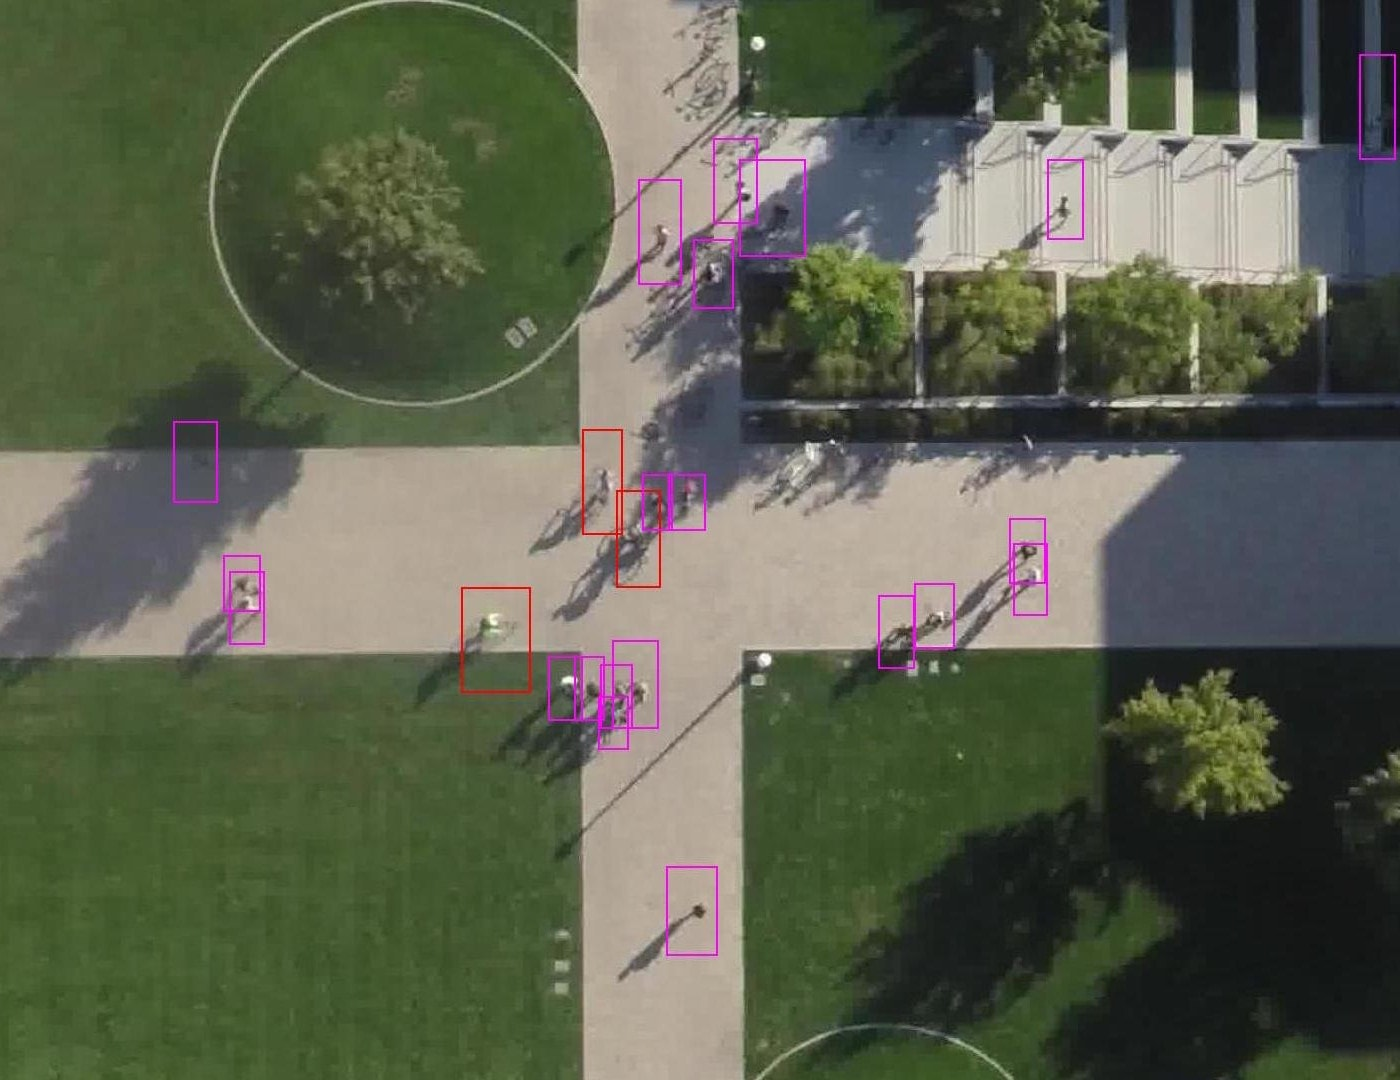
\includegraphics[width=.49\linewidth]{images/dataset_3.jpg}
        \caption{Ukázka z použitého datasetu.}
    \end{figure}

\end{frame}

%%%%%%%%%%%%%%%%%%%%%%%%%%%%%%%%%%%%%%%%%%%%%%%%%%%%%%%%%%%%%%%%%%

% \begin{frame}\frametitle{Přesnost detektoru}
    
%     \begin{itemize}
%         \item Nejvyšší přesnost kolem 40. epochy -- 58\,\%.
%     \end{itemize}    
    
%     \begin{figure}[H]
%         \centering
%         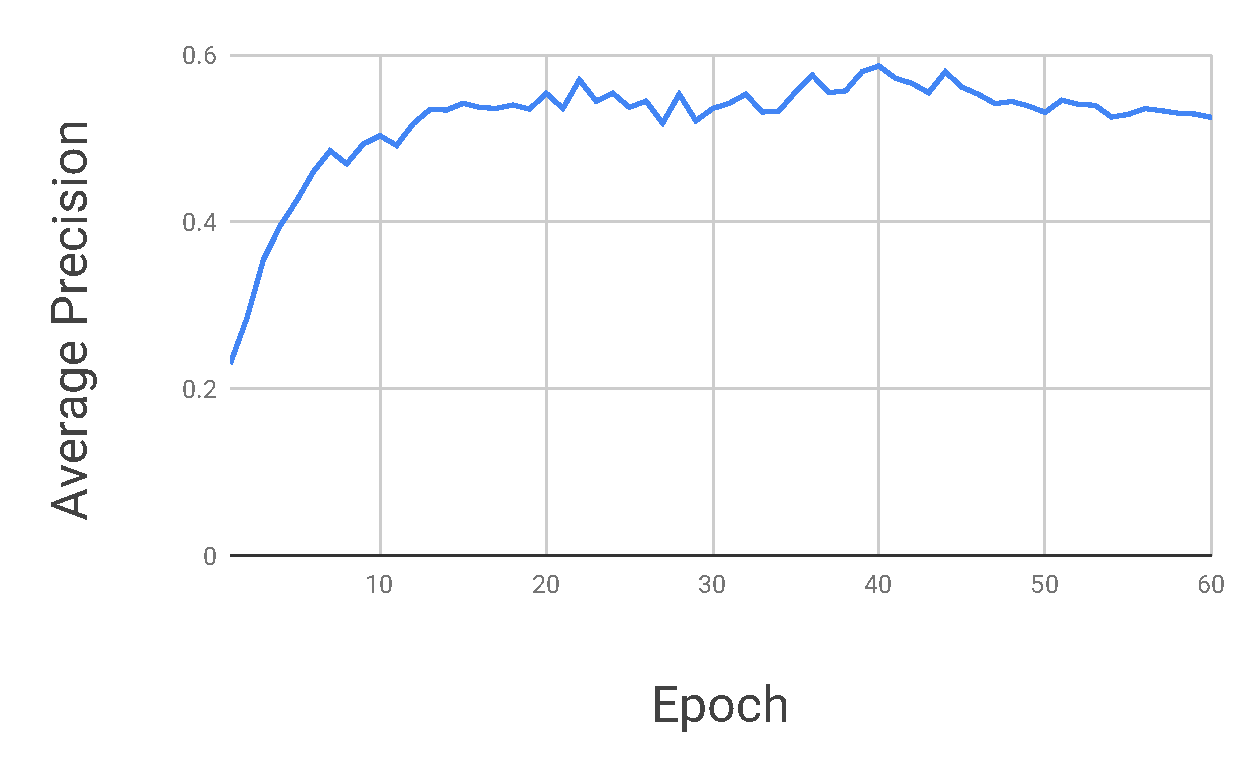
\includegraphics[width=.9\linewidth]{images/average-precision.pdf}
%         \caption{Přesnost detektoru na validačních datech.}
%     \end{figure}
    
% \end{frame}

%%%%%%%%%%%%%%%%%%%%%%%%%%%%%%%%%%%%%%%%%%%%%%%%%%%%%%%%%%%%%%%%%%

\begin{frame}\frametitle{Výsledky detektoru}
    
     \begin{figure}[H]
        \centering
        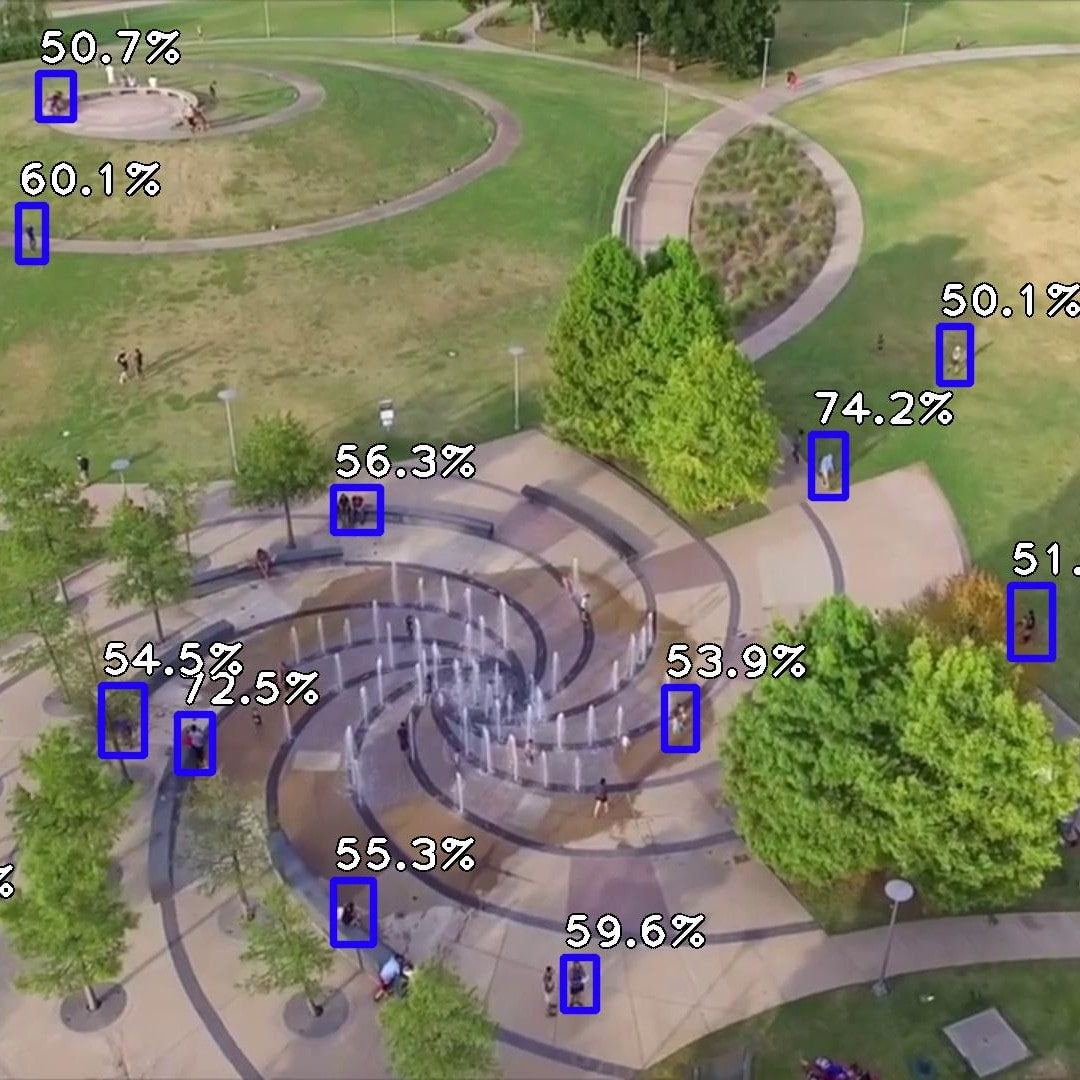
\includegraphics[width=.49\linewidth]{images/t3-t2.jpg}
        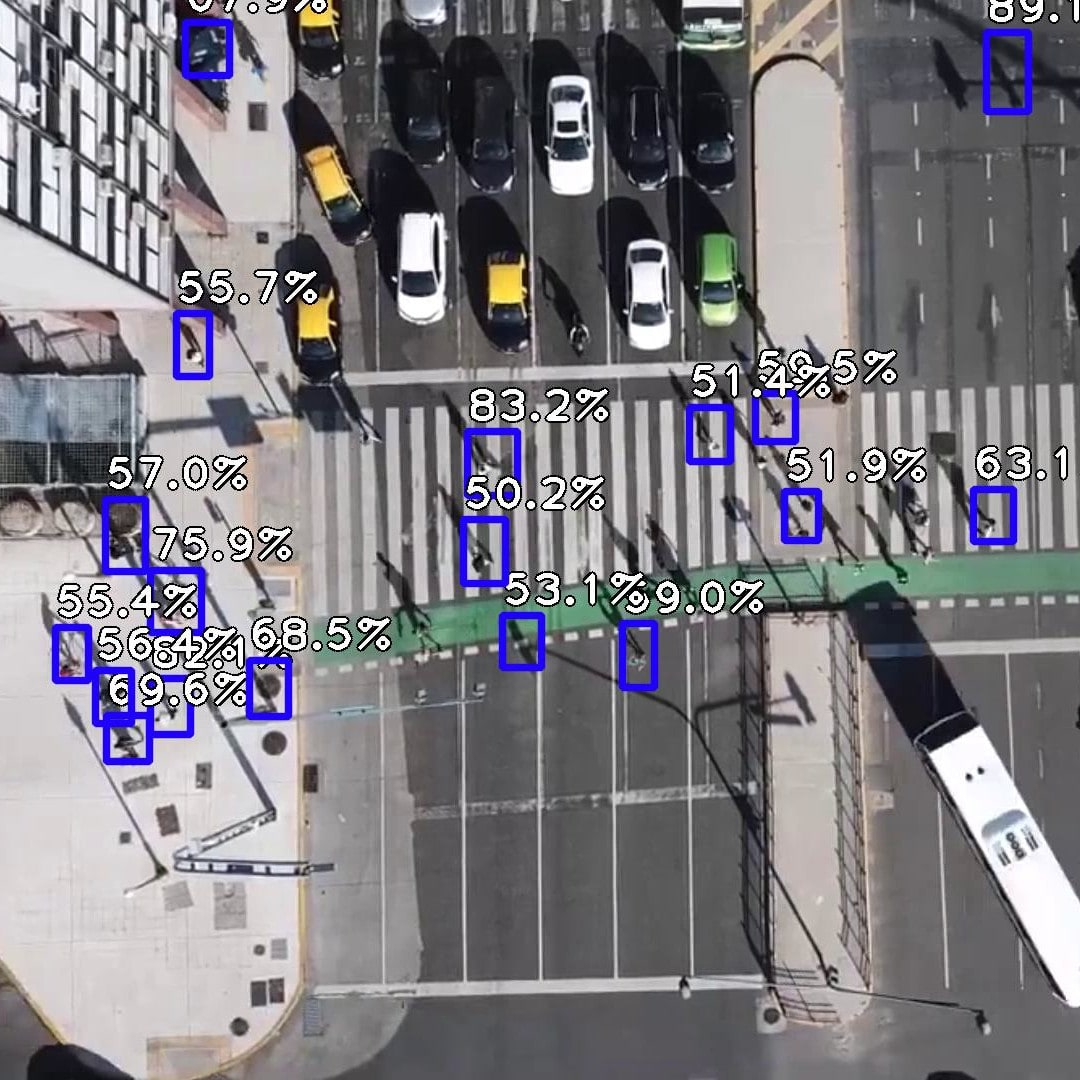
\includegraphics[width=.49\linewidth]{images/t3-t3.jpg}
        \caption{Výsledky detektoru na obrázcích, které nebyly součástí datasetu.}
    \end{figure}
    
\end{frame}

%%%%%%%%%%%%%%%%%%%%%%%%%%%%%%%%%%%%%%%%%%%%%%%%%%%%%%%%%%%%%%%%%%

% \begin{frame}\frametitle{Algoritmus identifikace osob}
    
%     \begin{itemize}
%         \item Video je po snímcích předáváno detektoru.
%         \item Detektor ve snímku rozpozná osoby.
%         \item Segmenty s detekovanými lidmi jsou z obrazu vyříznuty.
%         \item Z výřezů jsou extrahovány příznakové vektory.
%         \item Detekované osoby z aktuálního snímku jsou porovnávány s osobami již viděnými (přes jejich příznakové vektory).
%         \item Po zpracování celého videozáznamu, jsou vykresleny trajektorie pohybů do prvního snímku videa pro každou detekovanou osobu.
%     \end{itemize}    
    
% \end{frame}

%%%%%%%%%%%%%%%%%%%%%%%%%%%%%%%%%%%%%%%%%%%%%%%%%%%%%%%%%%%%%%%%%%

\begin{frame}\frametitle{Výsledná aplikace}
    
    \begin{figure}[H]
        \centering
        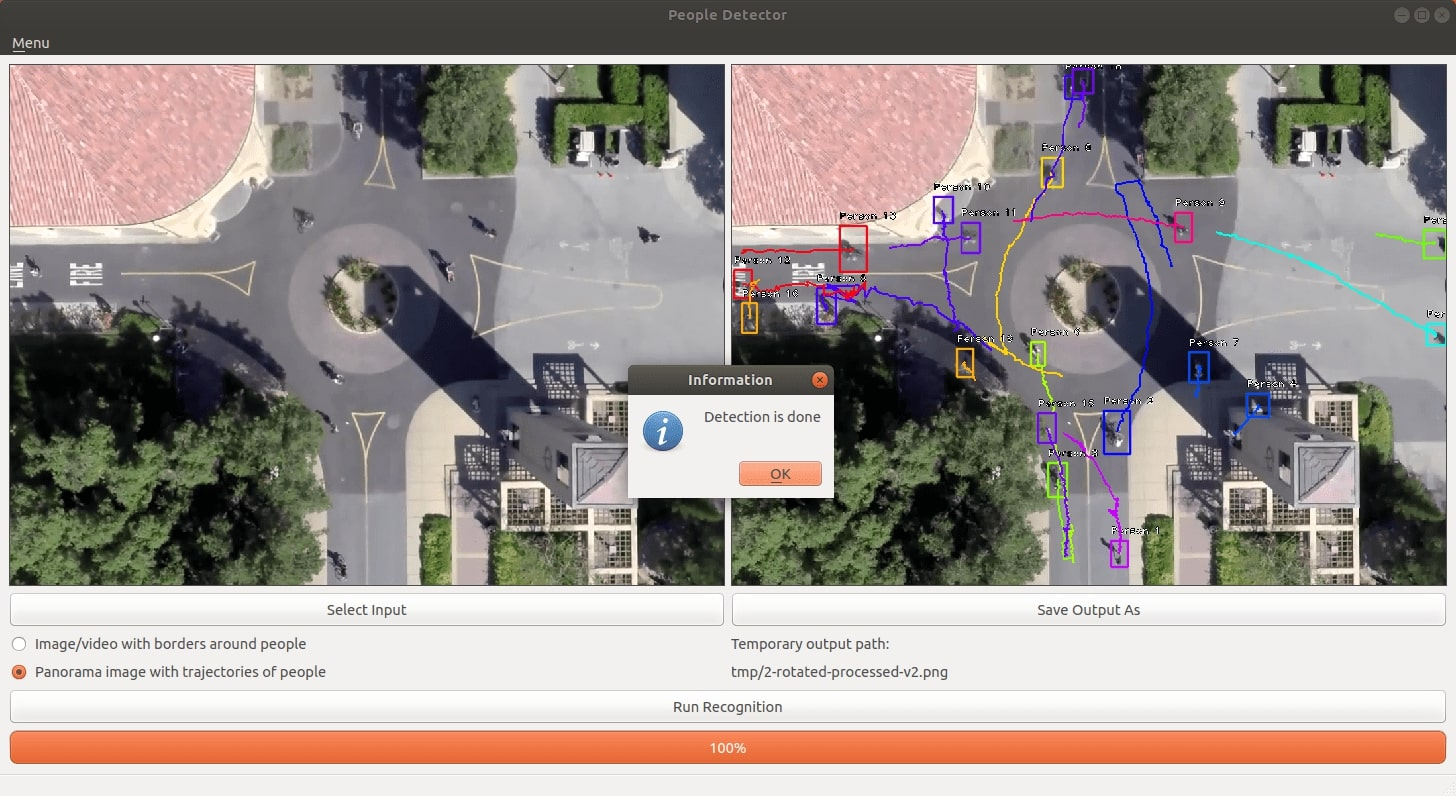
\includegraphics[width=.99\linewidth]{images/gui.jpg}
        \caption{Aplikace People Detector.}
    \end{figure}
    
\end{frame}

%%%%%%%%%%%%%%%%%%%%%%%%%%%%%%%%%%%%%%%%%%%%%%%%%%%%%%%%%%%%%%%%%%

\begin{frame}\frametitle{Video z validační části datasetu}
    
    \begin{figure}[H]
        \centering
        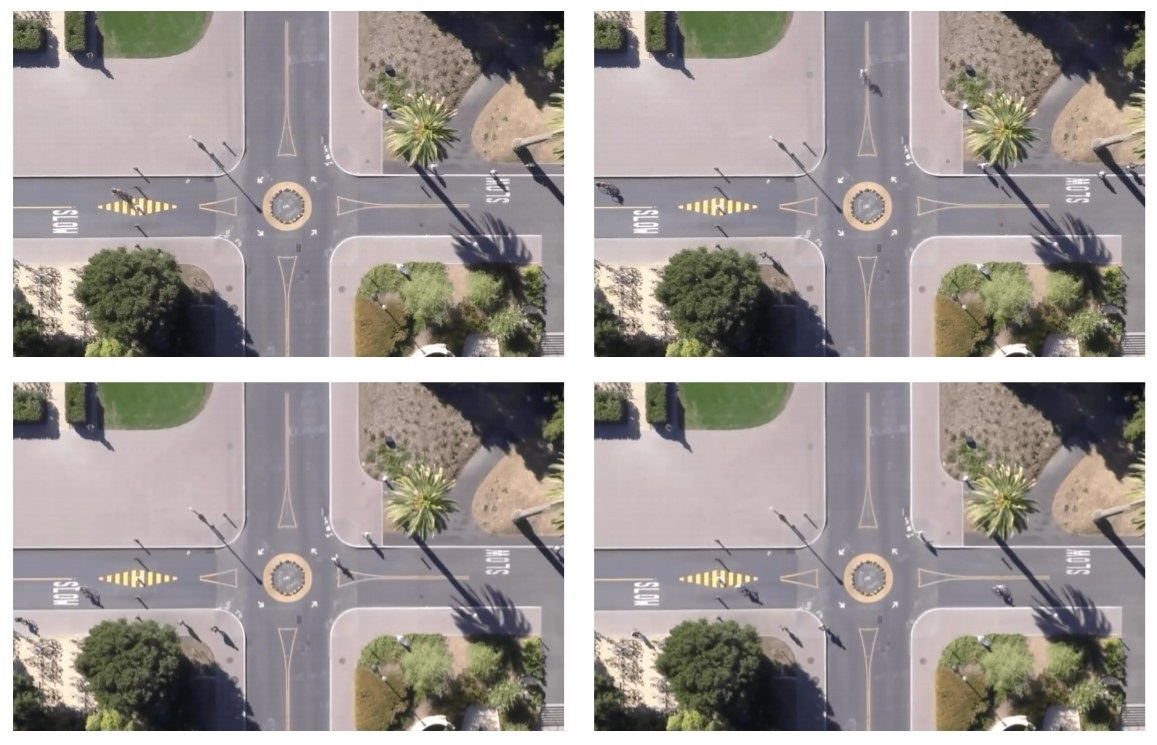
\includegraphics[width=.99\linewidth]{images/test1-input.jpg}
        \caption{Video z validační části datasetu.}
    \end{figure}
    
\end{frame}

%%%%%%%%%%%%%%%%%%%%%%%%%%%%%%%%%%%%%%%%%%%%%%%%%%%%%%%%%%%%%%%%%%

\begin{frame}\frametitle{Video z validační části datasetu -- výstup}
    
    \begin{figure}[H]
        \centering
        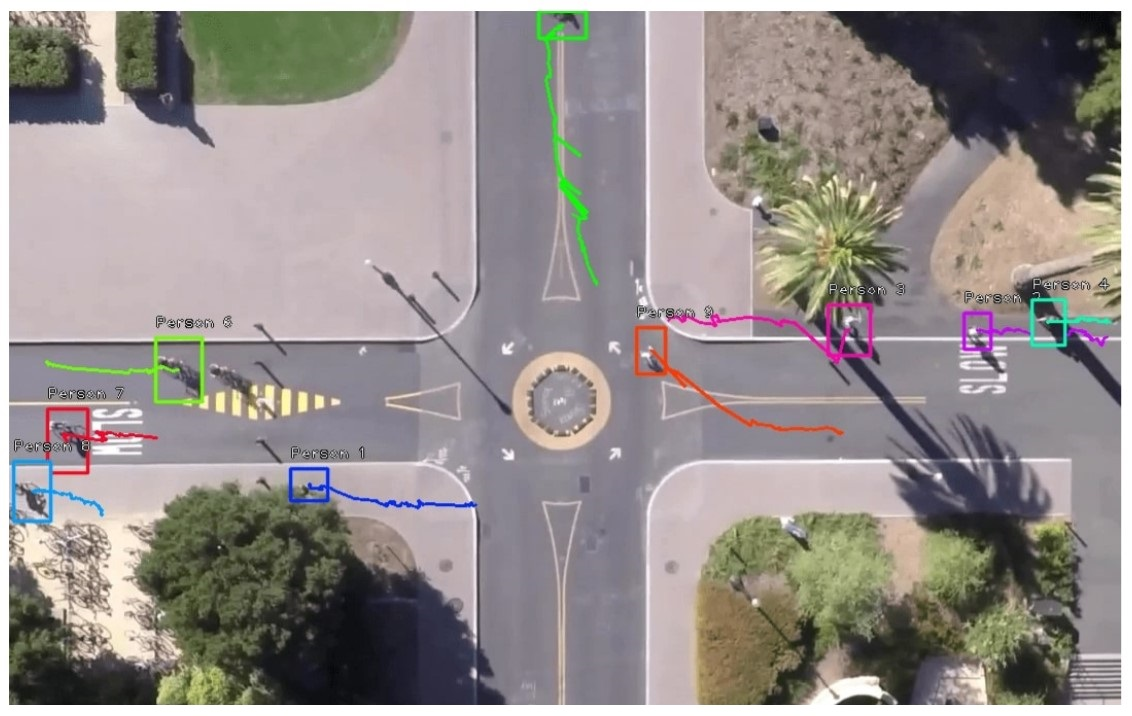
\includegraphics[width=.99\linewidth]{images/test1-output.jpg}
        \caption{Video z validační části datasetu -- výsledek.}
    \end{figure}
    
\end{frame}

%%%%%%%%%%%%%%%%%%%%%%%%%%%%%%%%%%%%%%%%%%%%%%%%%%%%%%%%%%%%%%%%%%

\begin{frame}\frametitle{Video pořízené dronem}
    
    \begin{figure}[H]
        \centering
        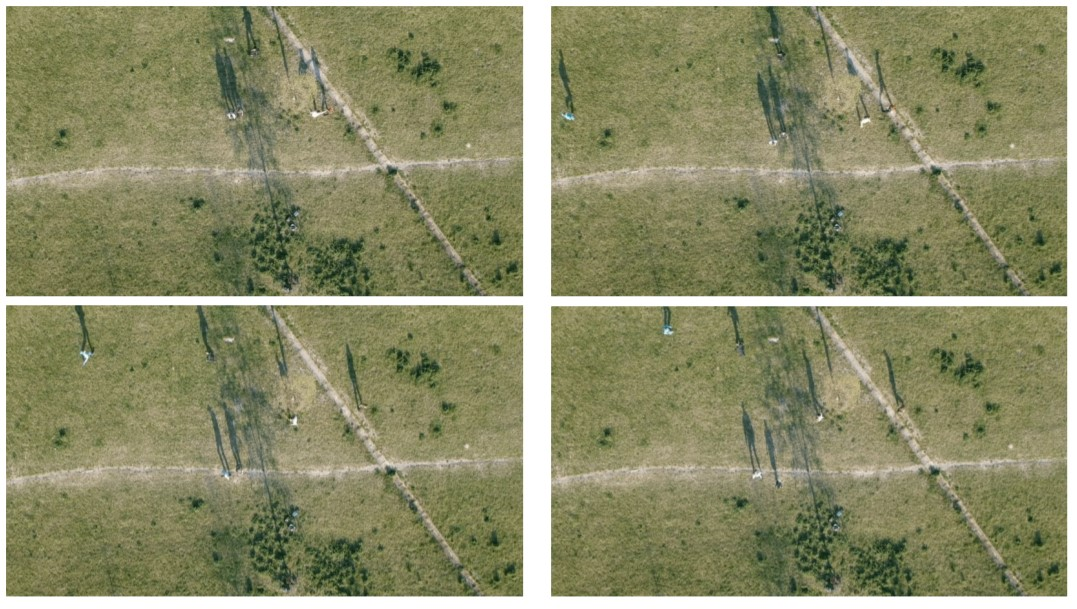
\includegraphics[width=.99\linewidth]{images/test2-input.jpg}
        \caption{Video pořízené dronem.}
    \end{figure}
    
\end{frame}

%%%%%%%%%%%%%%%%%%%%%%%%%%%%%%%%%%%%%%%%%%%%%%%%%%%%%%%%%%%%%%%%%%

\begin{frame}\frametitle{Video pořízené dronem -- výstup}
    
    \begin{figure}[H]
        \centering
        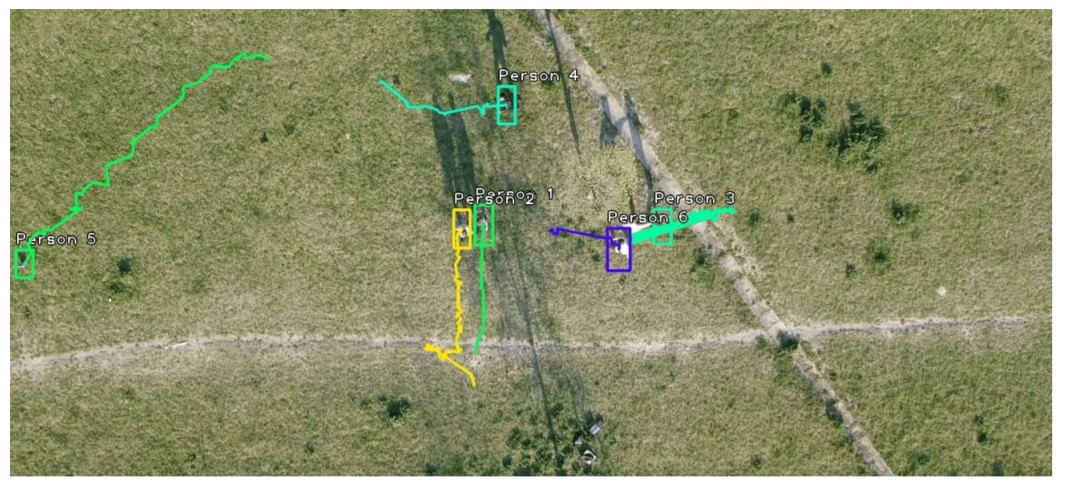
\includegraphics[width=.99\linewidth]{images/test2-output.jpg}
        \caption{Video pořízené dronem -- výsledek.}
    \end{figure}
    
\end{frame}

%%%%%%%%%%%%%%%%%%%%%%%%%%%%%%%%%%%%%%%%%%%%%%%%%%%%%%%%%%%%%%%%%%

\bluepage{Děkuji za pozornost.}

\appendix

\begin{frame}\frametitle{Otázka od oponenta}
    \begin{enumerate}
        \item Jaké musí být minimální rozlišení snímku osoby (z horního pohledu), aby detektor začal provádět úspěšné detekce?
    \end{enumerate}                
\end{frame}

\begin{frame}\frametitle{Otázka od oponenta}
    \begin{figure}[H]
        \centering
        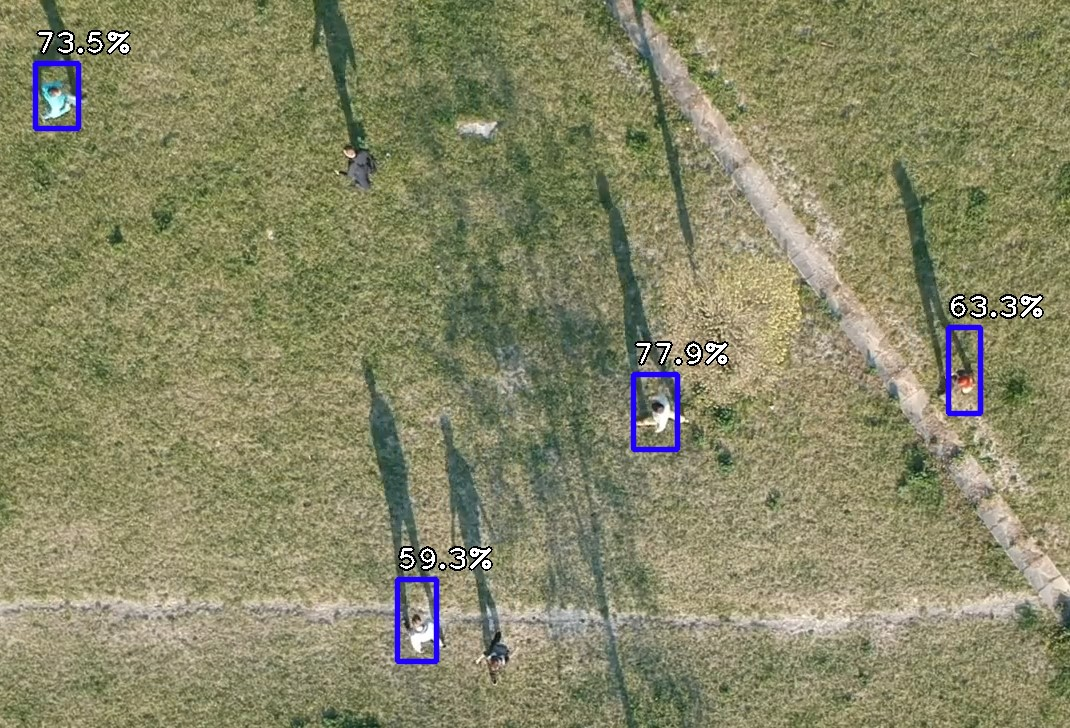
\includegraphics[width=.9\linewidth]{images/oponent-100.jpg}
        \caption{Snímek $1280 \times 720$\,px, osoba zachycena na $60 \times 40$\,px, detekováno 4/6.}
    \end{figure}                
\end{frame}

\begin{frame}\frametitle{Otázka od oponenta}
    \begin{figure}[H]
        \centering
        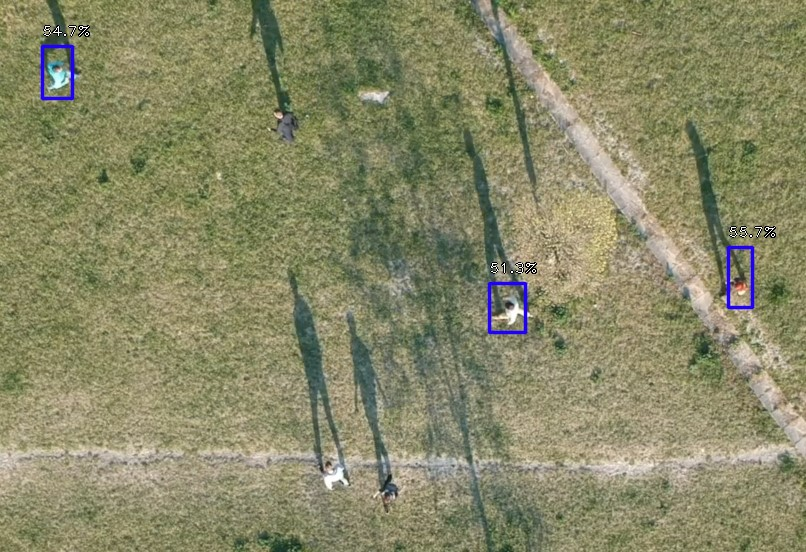
\includegraphics[width=.9\linewidth]{images/oponent-75.jpg}
        \caption{Snímek $960 \times 540$\,px, osoba zachycena na $45 \times 30$\,px, detekováno 3/6.}
    \end{figure}                
\end{frame}

\begin{frame}\frametitle{Otázka od oponenta}
    \begin{figure}[H]
        \centering
        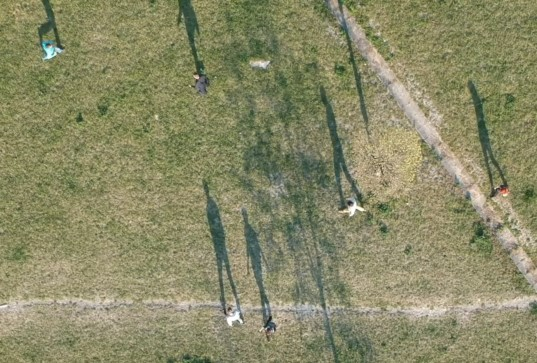
\includegraphics[width=.9\linewidth]{images/oponent-50.jpg}
        \caption{Snímek $640 \times 360$\,px, osoba zachycena na $30 \times 15$\,px, detekováno 0/6.}
    \end{figure}                
\end{frame}

\begin{frame}\frametitle{Otázka od oponenta}
     \begin{figure}[H]
        \centering
        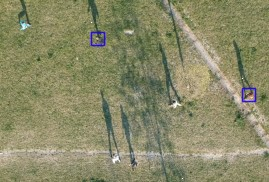
\includegraphics[width=.9\linewidth]{images/oponent-25.jpg}
        \caption{Snímek $320 \times 180$\,px, osoba zachycena na $15 \times 10$\,px, detekováno 2/6.}
    \end{figure} 
\end{frame}

\begin{frame}\frametitle{Otázka od oponenta}
    \begin{itemize}
        \item Nelze jednoznačně určit od jakého rozlišení bude detektor fungovat.
        \item Optimální záznam osoby může být kolem $2500$\,px.
            \item Pro více, či méně detailní záběry bude přesnost detektoru pravděpodobně klesat.
    \end{itemize}     
     
         
\end{frame}

%%%%%%%%%%%%%%%%%%%%%%%%%%%%%%%%%%%%%%%%%%%%%%%%%%%%%%%%%%%%%%%%%%

\end{document}

%%%%%%%%%%%%%%%%%%%%%%%%%%%%%%%%%%%%%%%%%%%%%%%%%%%%%%%%%%%%%%%%%%
